\documentclass{beamer}

\usepackage[spanish]{babel}
\usepackage{booktabs}

\usepackage[backend=biber, style=apa]{biblatex}   % misma bibliografia y estilo que la tesis
\addbibresource{../tesis/bibliografia.bib}

\graphicspath{{../replicacion/output/graficos/}}

\title{Efectos competitivos de la entrada y dispersión de precios en mercados locales}
\author{Joaquín Martínez}
\institute{Universidad de Chile, Facultad de Economía y Negocios}
\date{\today}

\begin{document}

\frame{\titlepage}

\begin{frame}{Motivación}
  \begin{itemize}
    \item La FNE sostiene que la competencia entre estaciones de servicio es local y que la presión competitiva deja de ser relevante a cierta distancia \parencite{FNE2021informe}.
    \begin{itemize}
      \item ¿Cuánto cae el precio de las incumbentes cuando abre una competidora?
      \item ¿A qué distancia deja de ser relevante ese efecto?
    \end{itemize}
    \item En Chile la transparencia de precios elevó los márgenes \parencite{LUCO2019}.
    \begin{itemize}
      \item ¿En qué parte de la distribución de precios del mercado se concentra?
    \end{itemize}
  \end{itemize}
\end{frame}

\begin{frame}{Contribución}
  \begin{itemize}
    \item \textbf{Transparencia y competencia:} la entrada desplaza la distribución hacia abajo por su cola izquierda.
    \item \textbf{Política de competencia:}
      \begin{itemize}
        \item evidencia para el radio de 3 km que usa la FNE como mercado relevante.
        \item cuantifica el costo de las barreras a la entrada por limitaciones del uso de suelo.
      \end{itemize}
  \end{itemize}
\end{frame}

\section{Mercado y datos}

\begin{frame}{Mercado y datos}
  \begin{itemize}
    \item Tres mayoristas integradas concentran tres cuartos de la distribución minorista.
    \item Precio en consignación (lo fija la mayorista) o concesión (la estación).
    \item MEPCO: referencia mayorista nacional y semanal, sin diferenciación geográfica.
  \end{itemize}
  \vfill
  \begin{itemize}
    \item \textbf{Datos:} precios de todas las estaciones en bencinaenlinea.cl, 2012--2026, con ubicación y marca, costo mayorista con MEPCO (Hacienda).
    \item Panel semanal (jueves a miércoles) colapsado a mensual.
    \item Entrada = primera aparición de una estación en el registro.
  \end{itemize}
\end{frame}

\begin{frame}{Precios promedio, 2012--2026}
  \centering
  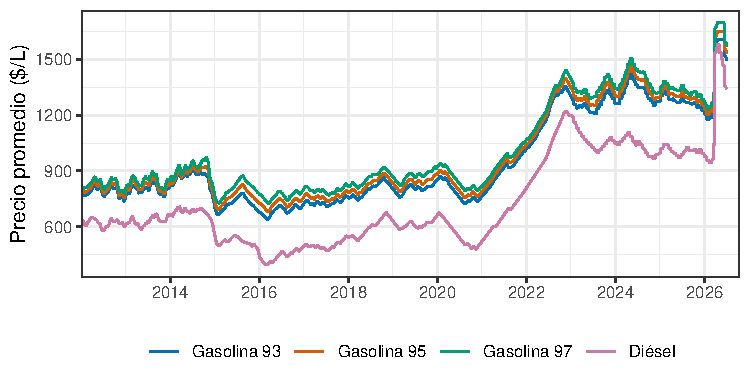
\includegraphics[width=\textwidth,height=0.85\textheight,keepaspectratio]{serie_precios.pdf}
\end{frame}

\begin{frame}{¿Por qué precios y no márgenes?}
  \centering
  \resizebox{\textwidth}{!}{\begin{tabular}{lcccccc}
\toprule
 & \multicolumn{2}{c}{Copec} & \multicolumn{2}{c}{Petrobras} & \multicolumn{2}{c}{Shell} \\
\cmidrule(lr){2-3} \cmidrule(lr){4-5} \cmidrule(lr){6-7}
Anillo & Este trabajo & FNE & Este trabajo & FNE & Este trabajo & FNE \\
\midrule
0--1 km & 9.4\% (62) & 5--10\% (40--50) & -- & -- & 9.4\% (62) & 0--5\% (20--30) \\
1--2 km & 9.9\% (66) & 5--10\% (50--60) & -- & -- & 9.5\% (63) & 0--5\% (20--30) \\
2--3 km & 10.4\% (69) & 5--10\% (40--50) & 9.6\% (63) & 0--5\% (20--30) & 10.6\% (71) & 0--5\% (20--30) \\
3--4 km & 10.7\% (71) & 5--10\% (40--50) & 11.0\% (74) & 0--5\% (20--30) & 10.2\% (68) & 0--5\% (20--30) \\
4--5 km & 12.2\% (83) & 5--10\% (50--60) & 10.2\% (68) & 5--10\% (30--40) & 10.5\% (71) & 0--5\% (20--30) \\
\bottomrule
\end{tabular}
}
  \vfill
  \footnotesize
  \begin{itemize}
    \item Margen con MEPCO (precio $-$ costo mayorista) frente al margen contable de la \textcite{FNE2021informe} en torno a la ex estación Sesa de Av. Tobalaba, agosto 2018 a julio 2019. Entre paréntesis, \$/L.
    \item Con MEPCO el margen es parecido entre marcas (62 a 83 \$/L). El contable es menor: unos 20 \$/L en Copec y 40 en Shell y Petrobras.
    \item El MEPCO omite flete, almacenamiento y diferencias de costo de adquisición: sobrestima el margen y oculta diferencias entre compañías.
    \item Por eso se estima sobre precios; los efectos fijos de marca $\times$ año absorben esas diferencias de costo.
  \end{itemize}
\end{frame}

\begin{frame}{Tratamiento y control}
  \begin{columns}
    \column{0.5\textwidth}
    \begin{itemize}
      \item \textbf{Tratada:} entrada de otra marca a 1 o 2 km.
      \item \textbf{Excluida:} entrada entre 2 y 3 km.
      \item \textbf{Control estricto:} nunca una entrada a menos de 5 km.
    \end{itemize}
    \column{0.6\textwidth}
    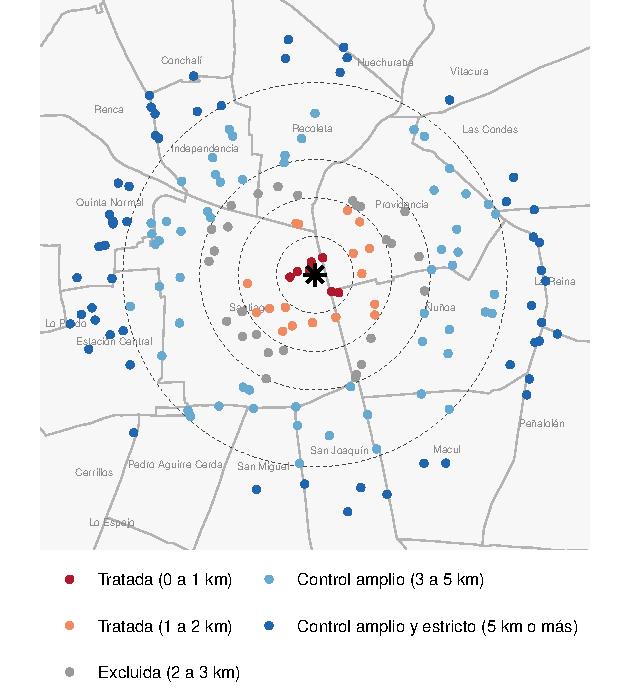
\includegraphics[width=\textwidth,height=1\textheight,keepaspectratio]{caso_entrada.pdf}
  \end{columns}
\end{frame}

\begin{frame}{Modelo}
  Modelo circular de \textcite{SALOP1979} aplicado a la venta minorista de combustibles por \textcite{CLEMENZGUGLER2006}.
  Precio de equilibrio simétrico:
  \[
    P^{*} = c + \beta\, 2^{1-\beta}\, \tau\, (n/L)^{-\beta},
    \qquad \frac{\partial P^{*}}{\partial n} < 0
  \]
  \begin{itemize}
    \item $n$: estaciones idénticas y equidistantes en un círculo de largo $L$.
    \item $c$: costo marginal, común a todas las estaciones.
    \item Un consumidor en $Z_j$ que compra en la estación $z_i$ paga un costo de transporte $\tau \left| Z_j - z_i \right|^{\beta}$:
      \begin{itemize}
        \item $\tau > 0$: escala del costo de transporte.
        \item $\beta \geq 1$: curvatura del costo ($\beta = 1$ lineal, $\beta = 2$ cuadrático).
      \end{itemize}
    \item Más estaciones en el mismo espacio $\Rightarrow$ menor precio.
  \end{itemize}
\end{frame}

\begin{frame}{Hipótesis}
  \begin{enumerate}
    \item \textbf{Efecto disciplinador:} la entrada reduce el precio de las incumbentes.
    \item \textbf{Atenuación espacial:} el efecto decrece con la distancia y se anula desde un umbral.
    \item \textbf{Asimetría distributiva:} el desplazamiento se concentra en la parte baja de la distribución de precios.
  \end{enumerate}
\end{frame}

\section{Identificación}

\begin{frame}{Estrategia de identificación}
  Estudio de eventos escalonado sobre el panel mensual:
  \[
    p_{it} = \alpha_i + \lambda_t + \gamma_{r(i)a(t)} + \delta_{m(i)a(t)}
    + \sum_{\tau \neq -1} \beta_\tau D^{\tau}_{it} + \varepsilon_{it}
  \]
  \begin{itemize}
    \item $p_{it}$: log del precio $\times$ 100, bins de seis meses, extremos agrupados.
    \item Efectos fijos de estación, mes, región $\times$ año y marca $\times$ año.
    \item Supuesto: dada la ubicación, el \emph{momento} de la entrada es exógeno a los precios de las incumbentes \parencite{ARCIDIACONO2020,FISCHER2025}.
    \item TWFE y \textcite{SUNABRAHAM2021}, errores agrupados por comuna.
  \end{itemize}
\end{frame}

\section{Resultados}

\begin{frame}{H1: la entrada reduce el precio de las incumbentes}
  \centering
  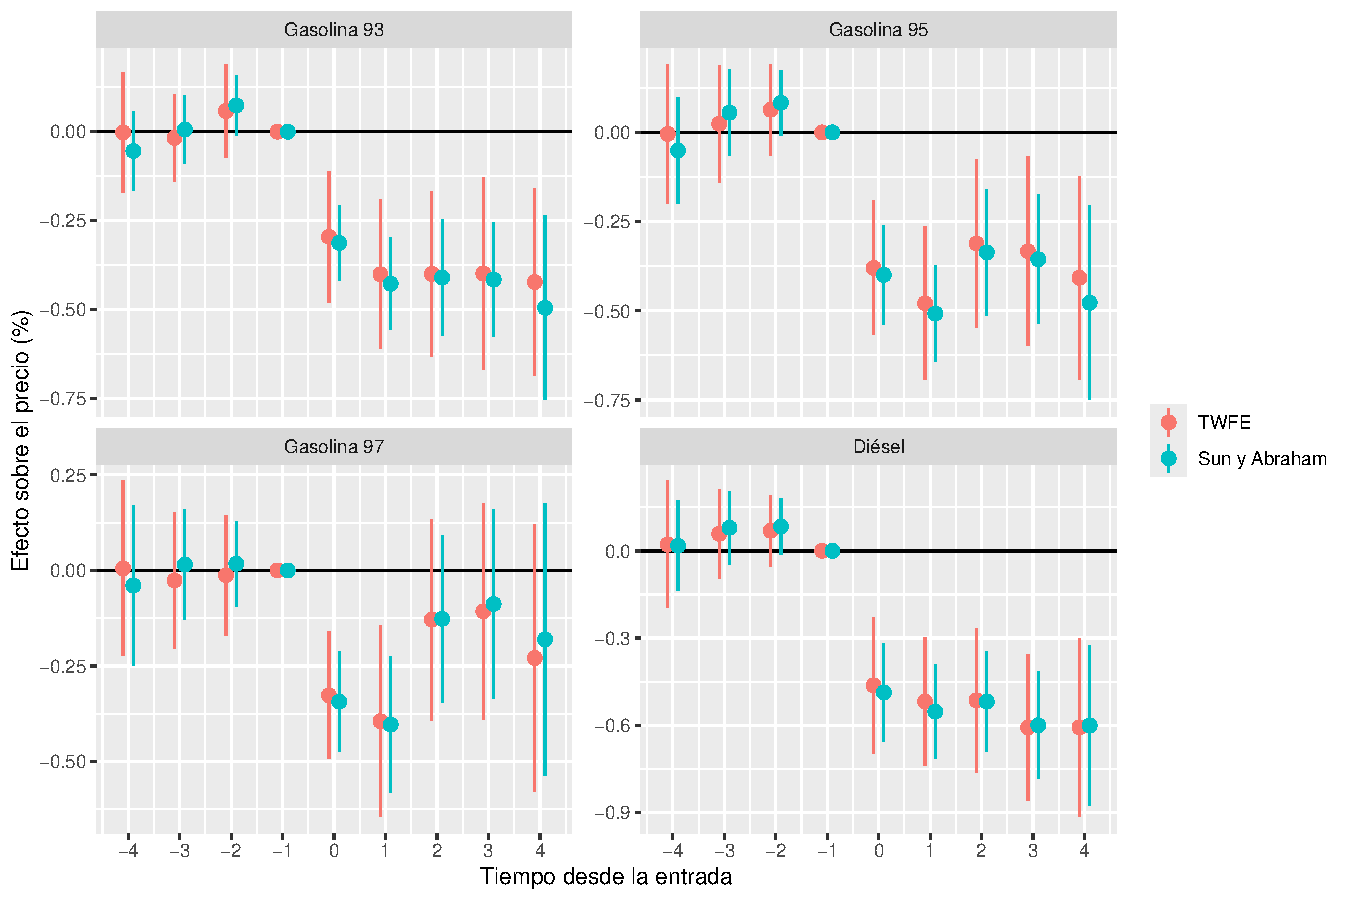
\includegraphics[width=\textwidth,height=0.75\textheight,keepaspectratio]{sunab_2012_2026.pdf}
  \small Efecto promedio: 0,40\% en 93 y 95, 0,24\% en 97 y 0,59\% en diésel (unos 4 \$/L).
\end{frame}

\begin{frame}{H2: el efecto se atenúa con la distancia}
  \centering
  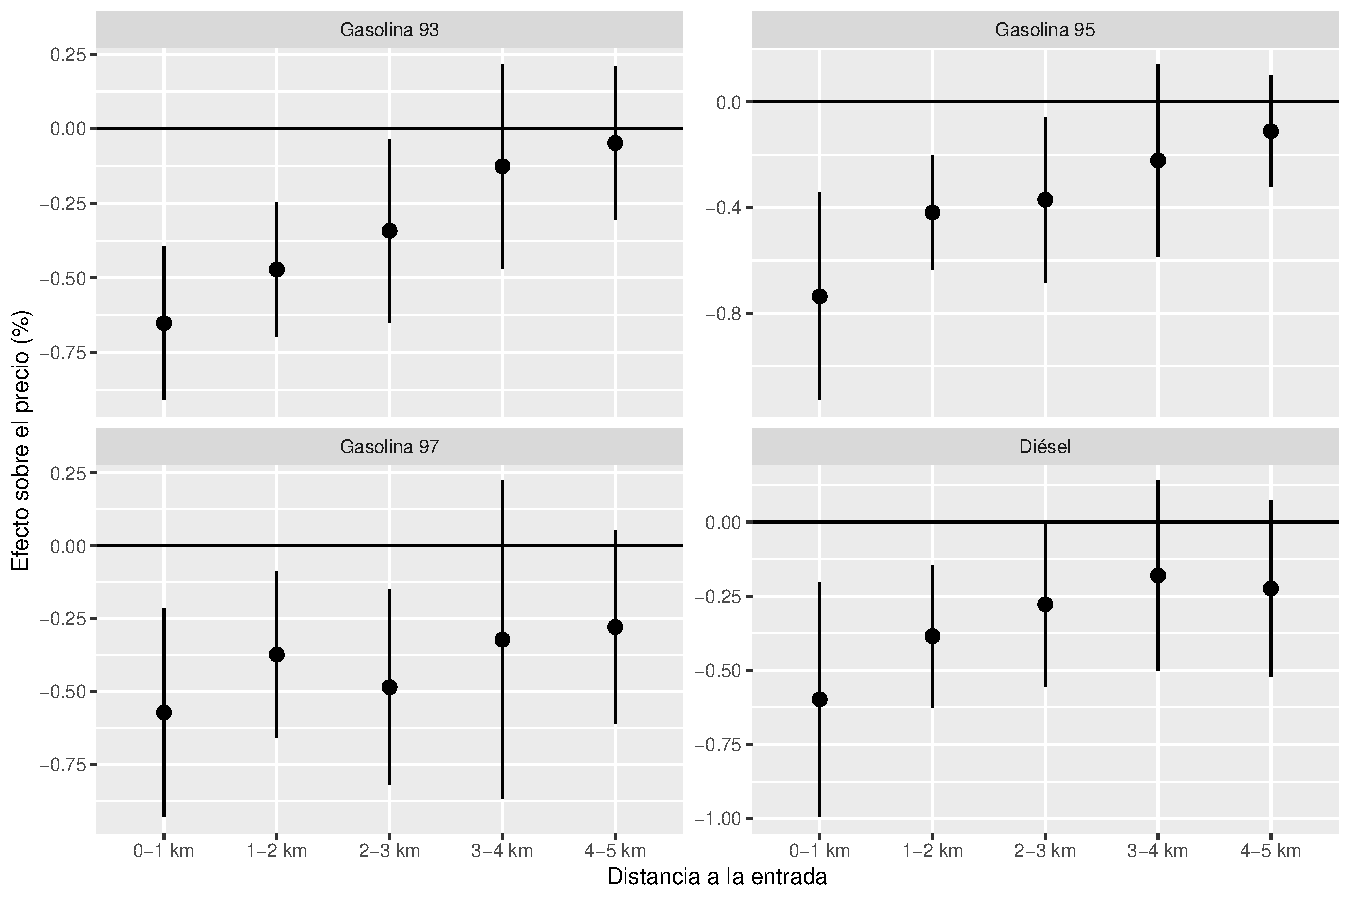
\includegraphics[width=\textwidth,height=0.75\textheight,keepaspectratio]{atenuacion_distancia.pdf}
  \small Significativo hasta 3 km en los cuatro combustibles, nulo entre 3 y 5 km.
\end{frame}

\begin{frame}{H2: sin efecto en estaciones de autopista}
  \centering
  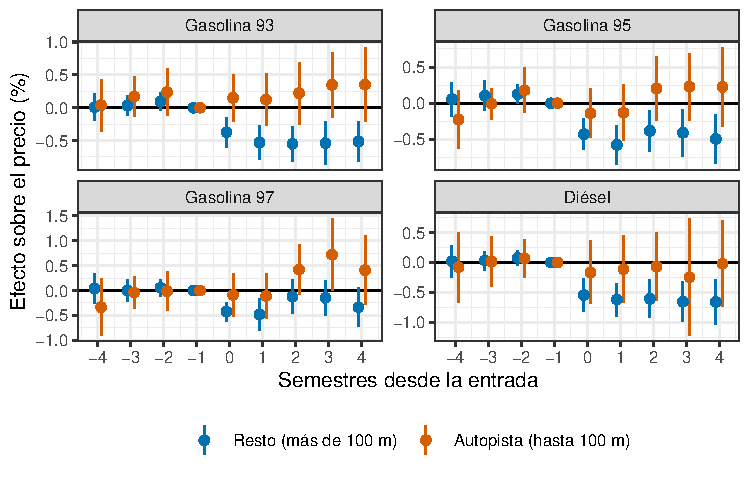
\includegraphics[width=\textwidth,height=0.75\textheight,keepaspectratio]{het_autopista.pdf}
  \small Su mercado relevante es el corredor vial, no el radio en torno a ellas.
\end{frame}

\begin{frame}{H3: caen más los precios bajos del mercado}
  \centering
  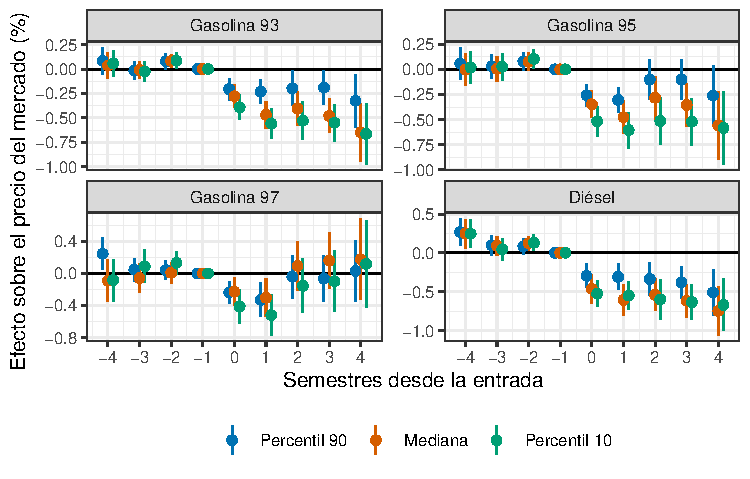
\includegraphics[width=\textwidth,height=0.75\textheight,keepaspectratio]{mercado.pdf}
  \small Estudio de eventos de \textcite{SUNABRAHAM2021} sobre cuantiles de los precios del mercado local (2 km).
  La entrada aumenta la dispersión, la 97 es la excepción.
\end{frame}

\begin{frame}{H3: regresión de distribución}
  \textcite{CHERNOZHUKOV2013}:
  \begin{itemize}
    \item $\tilde{p}_{it}$: precio menos su media nacional del mes (\$/L).
    \item $c$: umbral de una grilla de 41 valores de $\tilde{p}_{it}$.
    \item Para cada umbral, una regresión con la especificación principal:
  \end{itemize}
  \[
    \mathbf{1}[\tilde{p}_{it} \leq c] = \beta(c)\, \text{Post}_{it} + \alpha_i + \lambda_t + \gamma_{r(i)a(t)} + \delta_{m(i)a(t)} + \varepsilon_{it}
  \]
  \begin{itemize}
    \item $\beta(c) > 0$: la entrada aumenta la masa de precios bajo $c$.
    \item Contrafactual: acumulada observada de las tratadas después de la entrada menos $\beta(c)$.
  \end{itemize}
\end{frame}

\begin{frame}{H3: la grilla de umbrales $c$}
  \begin{itemize}
    \item $c_k$ es el cuantil $q_k$ de $\tilde{p}_{it}$ en la muestra de estimación de cada combustible.
    \item $q_k = 2\%, 4{,}4\%, 6{,}8\%, \ldots, 98\%$: 41 valores separados por 2,4 puntos.
  \end{itemize}
  \vfill
  \centering
  \scriptsize
  \begin{tabular}{lccc}
    \toprule
    & \multicolumn{3}{c}{Umbral $c$ (\$/L)} \\
    \cmidrule(lr){2-4}
    & $q = 2\%$ & $q = 50\%$ & $q = 98\%$ \\
    \midrule
    Gasolina 93 & -56,1 & 5,2 & 66,3 \\
    Gasolina 95 & -59,4 & 6,2 & 56,6 \\
    Gasolina 97 & -70,4 & 6,1 & 55,0 \\
    Diésel      & -42,3 & 1,9 & 87,0 \\
    \bottomrule
  \end{tabular}
  \vfill
  \raggedright
  \begin{itemize}
    \item \textbf{Cuantiles y no valores fijos en \$/L:} la grilla sigue la distribución de cada combustible y entre dos umbrales consecutivos cae la misma proporción de observaciones, así $\beta(c)$ recorre toda la acumulada de forma pareja.
    \item \textbf{De 2 a 98:} fuera de ese rango los umbrales quedarían fijados por unos pocos precios atípicos y el indicador casi no varía.
  \end{itemize}
\end{frame}

\begin{frame}{H3: la base de la regresión de distribución}
  \centering
  \scriptsize
  \begin{tabular}{llcccccc}
    \toprule
    & & & & & \multicolumn{3}{c}{$\mathbf{1}[\tilde{p}_{it} \leq c]$} \\
    \cmidrule(lr){6-8}
    Estación & Mes & Post & Precio & $\tilde{p}_{it}$ & $c = -27{,}8$ & $c = 5{,}2$ & $c = 31{,}8$ \\
    \midrule
    Tratada & dic 2017 & 0 & 767 & 6,6   & 0 & 0 & 1 \\
    Tratada & ene 2018 & 1 & 760 & -3,3  & 0 & 1 & 1 \\
    Tratada & feb 2018 & 1 & 761 & -2,5  & 0 & 1 & 1 \\
    Control & dic 2017 & 0 & 733 & -27,4 & 0 & 1 & 1 \\
    Control & ene 2018 & 0 & 728 & -35,3 & 1 & 1 & 1 \\
    Control & feb 2018 & 0 & 738 & -25,5 & 0 & 1 & 1 \\
    \bottomrule
  \end{tabular}
  \vfill
  \begin{itemize}
    \item Gasolina 93. Tratada: co811006, con entrada en enero de 2018. Control: co840701.
    \item Media nacional: 760,4, 763,3 y 763,5 \$/L.
    \item Tres de los 41 umbrales: $c_4$, $c_{21}$ y $c_{38}$ ($q$ = 9,2\%, 50\% y 90,8\%).
    \item Cada columna $\mathbf{1}[\tilde{p}_{it} \leq c]$ es la variable dependiente de una regresión: 41 en total.
  \end{itemize}
\end{frame}

\begin{frame}{H3: distribución de precios con y sin entrada}
  \centering
  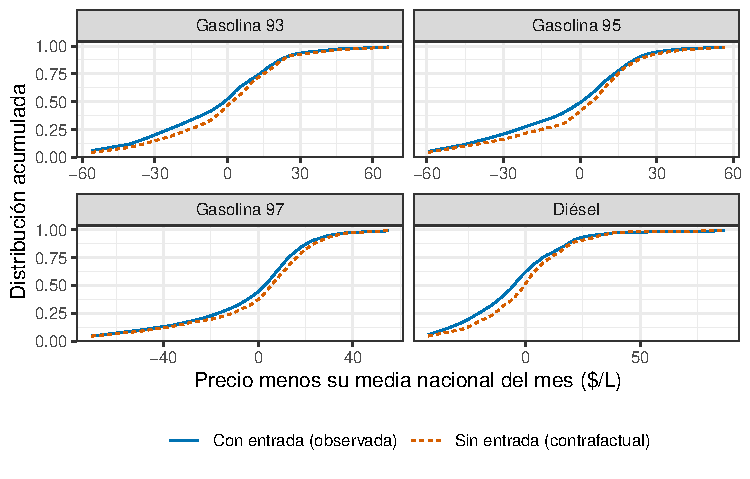
\includegraphics[width=\textwidth,height=0.75\textheight,keepaspectratio]{distribucion_acumulada.pdf}
  \small El desplazamiento hacia precios menores se concentra en la mitad baja de la distribución.
\end{frame}

\section{Robustez}

\begin{frame}{Robustez}
  \begin{itemize}
    \item \textbf{Tendencias paralelas} \parencite{RAMBACHAN2023}: el primer semestre resiste $\bar{M}$ entre 1 y 2,25 y va bajando con el tiempo.
    \item \textbf{Salida de incumbentes:} su número no cambia en el primer año.
    \item \textbf{Placebo adelantado:} el quiebre ocurre en la fecha registrada. Pequeña disminución no est. significativa el mes anterior.
    \item \textbf{Placebo en controles:} 500 réplicas, efecto medio entre 0,00\% y 0,02\%.
    \item \textbf{Ventanas:} efecto mayor en 2014--2019 y menor y menos persistente en 2021--2026 (anexo).
    \item Errores de \textcite{CONLEY1991}, panel semanal y grupo de control amplio: sin cambios.
  \end{itemize}
\end{frame}

\begin{frame}{Placebo: entrada adelantada seis meses}
  \centering
  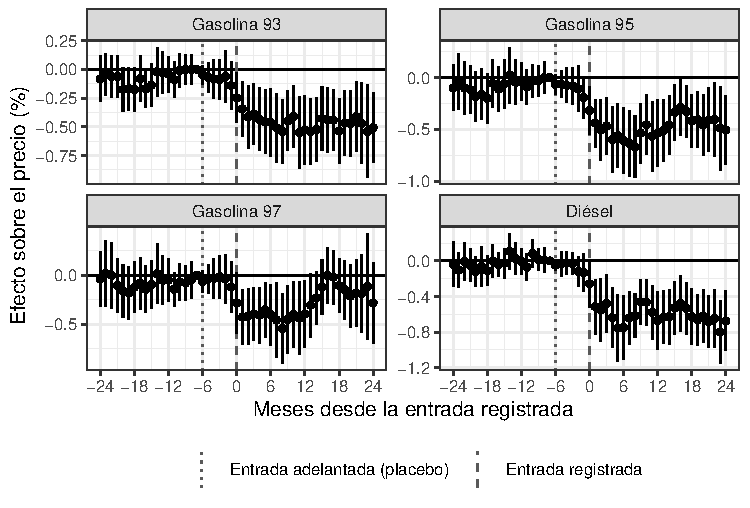
\includegraphics[width=\textwidth,height=0.85\textheight,keepaspectratio]{placebo_adelanto.pdf}
\end{frame}

\section{Conclusión}

\begin{frame}{Conclusiones}
  \begin{itemize}
    \item La entrada reduce el precio de las incumbentes a 2 km o menos, de forma persistente salvo en la 97.
    \item El efecto desaparece desde los 3 km, respalda el radio que usa la FNE, salvo en autopistas.
    \item Las barreras a la entrada tienen un costo de competencia, cada entrada que no ocurre deja unos 4 \$/L de margen a las incumbentes.
    \item La ganancia se concentra en las estaciones baratas y por tanto beneficia más a quien compara precios.
  \end{itemize}
  \vfill
  \textbf{Limitaciones}
  \begin{itemize}
    \item Exogeneidad del momento de la entrada no verificable directamente.
    \item Efecto post pandemia no se identifica. 
    \item Sin volúmenes de venta no hay manera de hacer un análisis de bienestar.
  \end{itemize}
\end{frame}

\begin{frame}[allowframebreaks]{Referencias}
  \printbibliography[heading=none]
\end{frame}

\appendix
\section{Anexo}

\begin{frame}{Estructura del precio a público, 2021}
  \centering
  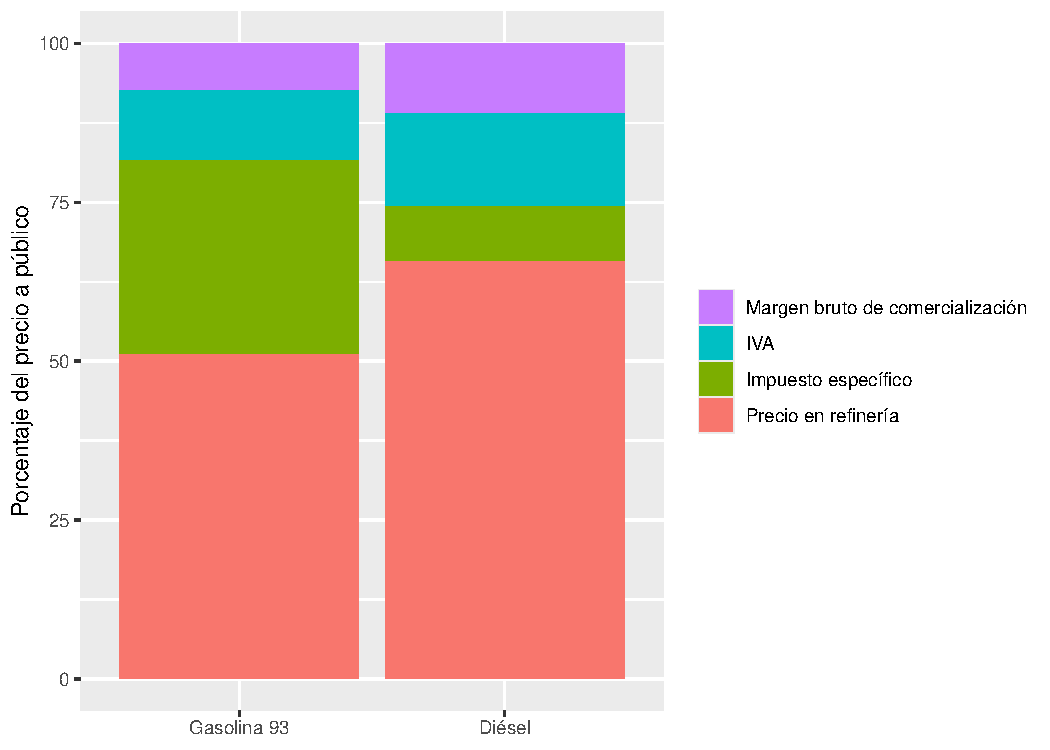
\includegraphics[width=\textwidth,height=0.8\textheight,keepaspectratio]{estructura_precios.pdf}
  \small Fuente: CNE. Promedio de los desgloses mensuales de 2021 para la Región Metropolitana.
\end{frame}

\begin{frame}{Escalera de efectos fijos, gasolina 93}
  \centering
  {\tiny 
\begingroup
\centering
\begin{tabular}{lccccc}
   \toprule
                        & (1)             & (2)            & (3)            & (4)            & (5)\\  
   \midrule 
   $\leq -4$            & -4.293$^{***}$  & 0.096          & 0.022          & -0.021         & -0.002\\   
                        & (1.308)         & (0.193)        & (0.148)        & (0.093)        & (0.086)\\   
   $-3$                 & -0.779          & 0.017          & 0.002          & -0.022         & -0.017\\   
                        & (1.108)         & (0.087)        & (0.082)        & (0.061)        & (0.062)\\   
   $-2$                 & -0.018          & 0.034          & 0.042          & 0.060          & 0.058\\   
                        & (0.814)         & (0.076)        & (0.070)        & (0.067)        & (0.067)\\   
   $0$                  & -1.146          & -0.374$^{***}$ & -0.357$^{***}$ & -0.316$^{***}$ & -0.296$^{***}$\\   
                        & (0.853)         & (0.106)        & (0.101)        & (0.096)        & (0.094)\\   
   $1$                  & -1.710          & -0.525$^{***}$ & -0.478$^{***}$ & -0.429$^{***}$ & -0.401$^{***}$\\   
                        & (1.152)         & (0.114)        & (0.100)        & (0.106)        & (0.107)\\   
   $2$                  & -2.152          & -0.562$^{***}$ & -0.493$^{***}$ & -0.430$^{***}$ & -0.400$^{***}$\\   
                        & (1.568)         & (0.145)        & (0.113)        & (0.119)        & (0.118)\\   
   $3$                  & -0.630          & -0.654$^{***}$ & -0.557$^{***}$ & -0.423$^{***}$ & -0.399$^{***}$\\   
                        & (1.653)         & (0.191)        & (0.156)        & (0.142)        & (0.138)\\   
   $\geq 4$             & 22.746$^{***}$  & -0.792$^{**}$  & -0.721$^{***}$ & -0.446$^{***}$ & -0.423$^{***}$\\   
                        & (1.741)         & (0.306)        & (0.173)        & (0.140)        & (0.135)\\   
   Tratada              & -10.704$^{***}$ & -1.598$^{***}$ &                &                &   \\   
                        & (1.739)         & (0.326)        &                &                &   \\   
   Tratadas             & 501             & 501            & 501            & 501            & 501\\  
   Controles            & 377             & 377            & 373            & 373            & 373\\  
    \\
   Observaciones        & 124,438         & 124,438        & 124,434        & 124,434        & 124,427\\  
    \\
   Mes                  & No              & Sí             & Sí             & Sí             & Sí\\  
   Estación             & No              & No             & Sí             & Sí             & Sí\\  
   Región $\times$ año  & No              & No             & No             & Sí             & Sí\\  
   Marca $\times$ año   & No              & No             & No             & No             & Sí\\  
   \bottomrule
\end{tabular}
\par\endgroup


}
\end{frame}

\begin{frame}{Escalera de efectos fijos, gasolina 97}
  \centering
  {\tiny 
\begingroup
\centering
\begin{tabular}{lccccc}
   \toprule
                        & (1)             & (2)            & (3)            & (4)            & (5)\\  
   \midrule 
   $\leq -4$            & -5.164$^{***}$  & 0.260          & 0.298          & 0.083          & 0.005\\   
                        & (1.118)         & (0.234)        & (0.190)        & (0.121)        & (0.117)\\   
   $-3$                 & -1.625$^{*}$    & 0.218$^{*}$    & 0.189$^{*}$    & 0.006          & -0.026\\   
                        & (0.918)         & (0.115)        & (0.114)        & (0.091)        & (0.091)\\   
   $-2$                 & -0.512          & 0.159          & 0.136          & -0.001         & -0.013\\   
                        & (0.753)         & (0.099)        & (0.095)        & (0.080)        & (0.080)\\   
   $0$                  & -0.626          & -0.375$^{***}$ & -0.377$^{***}$ & -0.320$^{***}$ & -0.327$^{***}$\\   
                        & (0.803)         & (0.098)        & (0.093)        & (0.088)        & (0.085)\\   
   $1$                  & -0.742          & -0.530$^{***}$ & -0.508$^{***}$ & -0.381$^{***}$ & -0.395$^{***}$\\   
                        & (1.010)         & (0.178)        & (0.166)        & (0.130)        & (0.128)\\   
   $2$                  & -1.162          & -0.285         & -0.236         & -0.110         & -0.129\\   
                        & (1.408)         & (0.179)        & (0.159)        & (0.134)        & (0.134)\\   
   $3$                  & 0.004           & -0.220         & -0.154         & -0.093         & -0.107\\   
                        & (1.544)         & (0.176)        & (0.149)        & (0.148)        & (0.144)\\   
   $\geq 4$             & 21.161$^{***}$  & -0.356         & -0.356$^{**}$  & -0.211         & -0.229\\   
                        & (1.679)         & (0.309)        & (0.179)        & (0.182)        & (0.178)\\   
   Tratada              & -10.126$^{***}$ & -1.430$^{***}$ &                &                &   \\   
                        & (1.664)         & (0.381)        &                &                &   \\   
   Tratadas             & 472             & 472            & 471            & 471            & 471\\  
   Controles            & 318             & 318            & 313            & 313            & 313\\  
    \\
   Observaciones        & 107,258         & 107,258        & 107,252        & 107,252        & 107,247\\  
    \\
   Mes                  & No              & Sí             & Sí             & Sí             & Sí\\  
   Estación             & No              & No             & Sí             & Sí             & Sí\\  
   Región $\times$ año  & No              & No             & No             & Sí             & Sí\\  
   Marca $\times$ año   & No              & No             & No             & No             & Sí\\  
   \bottomrule
\end{tabular}
\par\endgroup


}
\end{frame}

\begin{frame}{Escalera de efectos fijos, diésel}
  \centering
  {\tiny 
\begingroup
\centering
\begin{tabular}{lccccc}
   \toprule
                        & (1)             & (2)            & (3)            & (4)            & (5)\\  
   \midrule 
   $\leq -4$            & -3.616$^{*}$    & 0.183          & 0.099          & 0.044          & 0.022\\   
                        & (1.942)         & (0.275)        & (0.139)        & (0.121)        & (0.112)\\   
   $-3$                 & -0.077          & 0.144          & 0.114          & 0.060          & 0.059\\   
                        & (1.735)         & (0.103)        & (0.092)        & (0.077)        & (0.078)\\   
   $-2$                 & 0.691           & 0.108$^{*}$    & 0.096          & 0.070          & 0.069\\   
                        & (1.056)         & (0.063)        & (0.060)        & (0.062)        & (0.062)\\   
   $0$                  & -2.898$^{**}$   & -0.501$^{***}$ & -0.520$^{***}$ & -0.478$^{***}$ & -0.463$^{***}$\\   
                        & (1.290)         & (0.141)        & (0.132)        & (0.121)        & (0.119)\\   
   $1$                  & -4.550$^{**}$   & -0.576$^{***}$ & -0.553$^{***}$ & -0.542$^{***}$ & -0.518$^{***}$\\   
                        & (2.013)         & (0.140)        & (0.117)        & (0.111)        & (0.112)\\   
   $2$                  & -6.113$^{**}$   & -0.617$^{***}$ & -0.508$^{***}$ & -0.538$^{***}$ & -0.514$^{***}$\\   
                        & (2.624)         & (0.180)        & (0.130)        & (0.128)        & (0.126)\\   
   $3$                  & -4.353$^{*}$    & -0.723$^{***}$ & -0.549$^{***}$ & -0.628$^{***}$ & -0.608$^{***}$\\   
                        & (2.589)         & (0.200)        & (0.150)        & (0.134)        & (0.128)\\   
   $\geq 4$             & 27.296$^{***}$  & -0.947$^{***}$ & -0.628$^{***}$ & -0.666$^{***}$ & -0.608$^{***}$\\   
                        & (2.353)         & (0.304)        & (0.178)        & (0.165)        & (0.157)\\   
   Tratada              & -12.444$^{***}$ & -1.558$^{***}$ &                &                &   \\   
                        & (2.239)         & (0.409)        &                &                &   \\   
   Tratadas             & 506             & 506            & 506            & 506            & 506\\  
   Controles            & 385             & 385            & 383            & 383            & 383\\  
    \\
   Observaciones        & 126,402         & 126,402        & 126,400        & 126,400        & 126,393\\  
    \\
   Mes                  & No              & Sí             & Sí             & Sí             & Sí\\  
   Estación             & No              & No             & Sí             & Sí             & Sí\\  
   Región $\times$ año  & No              & No             & No             & Sí             & Sí\\  
   Marca $\times$ año   & No              & No             & No             & No             & Sí\\  
   \bottomrule
\end{tabular}
\par\endgroup


}
\end{frame}

\begin{frame}{Ventana 2014--2019}
  \centering
  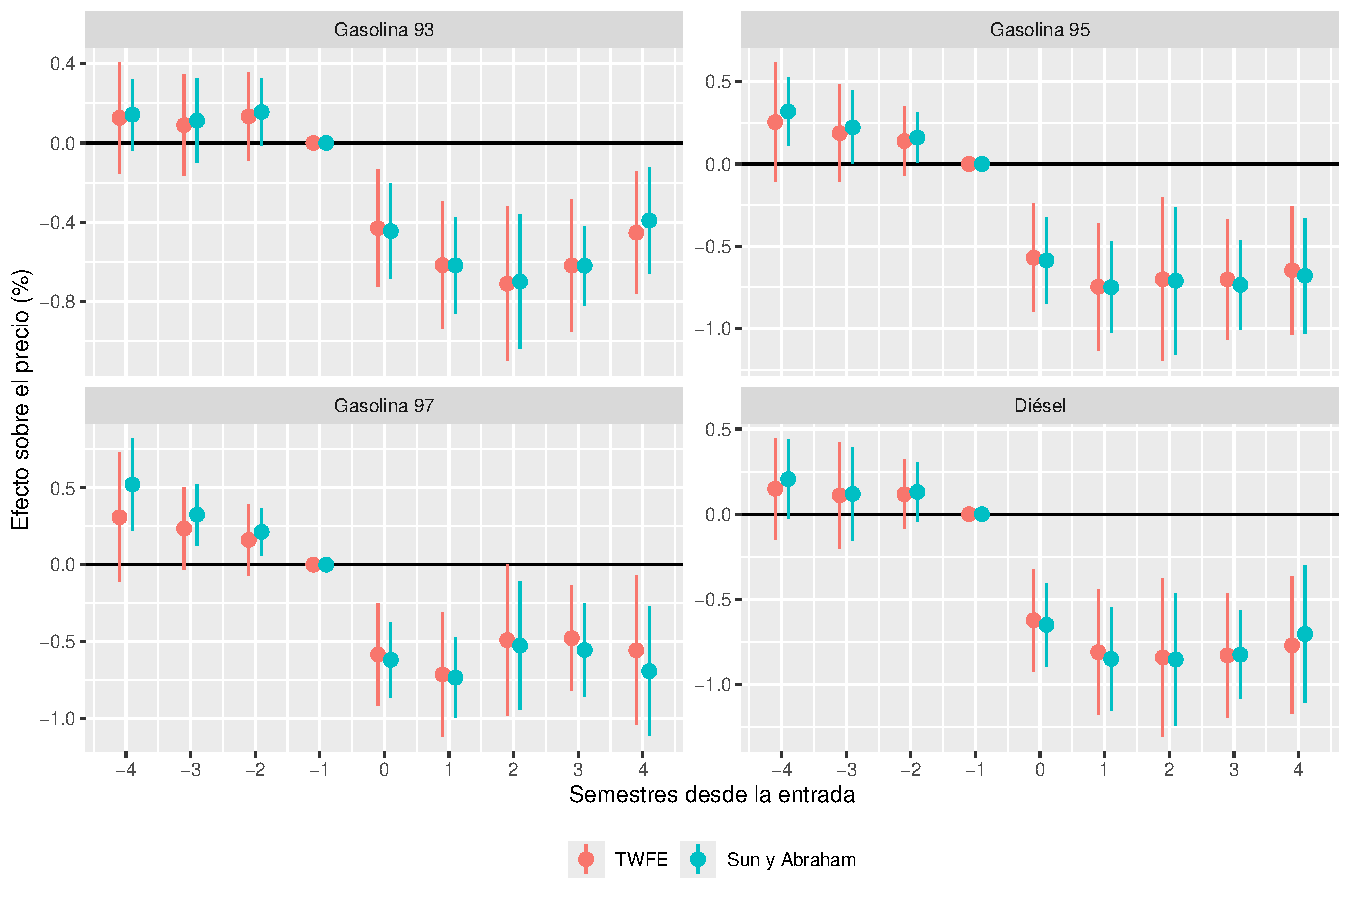
\includegraphics[width=\textwidth,height=0.8\textheight,keepaspectratio]{ventana_2014_2019.pdf}
  \small Incumbentes de 2014, cohortes de 2015 a 2019.
\end{frame}

\begin{frame}{Ventana 2021--2026}
  \centering
  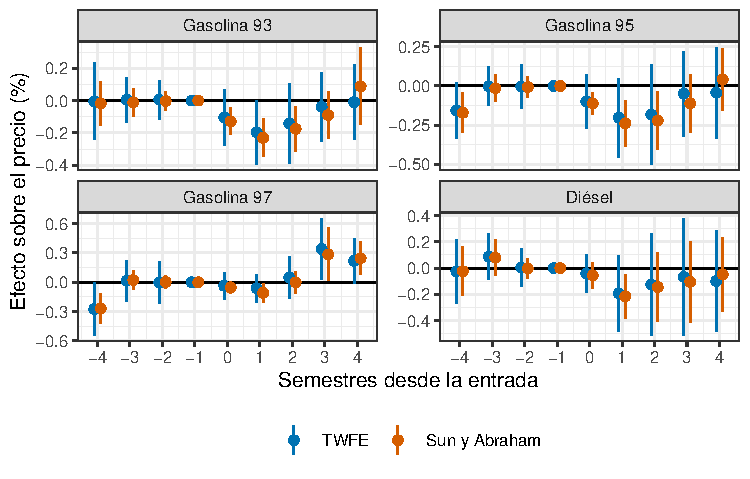
\includegraphics[width=\textwidth,height=0.8\textheight,keepaspectratio]{ventana_2021_2026.pdf}
  \small Incumbentes de 2021, cohortes de 2022 a febrero de 2026.
\end{frame}

\end{document}
